\section{Physics Modeling}\label{sec:physics}
The kinematics of the outgoing $\pi^0$ from CX interactions are not well known. The only existing differential cross section measurement on light nuclei from Ashery \textit{et.al.} \cite{Ashery2} is of 265 MeV$/c$ $\pi^{+}$ on oxygen. A comparison of this data and predictions from the \textsc{Neut} (v5.3.5) cascade model \cite{NEUT}, the \textsc{Geant4} (v9.04.04) Bertini cascade model \cite{bertini}, and the \textsc{Fluka} cascade model \cite{fluka1,fluka2} is shown in Fig. \ref{fig:pi0kinem}. The discrepancy among models is largest in the forward region, where CEMBALOS is most sensitive. In particular, the \textsc{Geant4} Bertini Cascade model used by our simulation shows the largest disagreement with data \cite{Ashery2}.

\begin{figure}[h]
 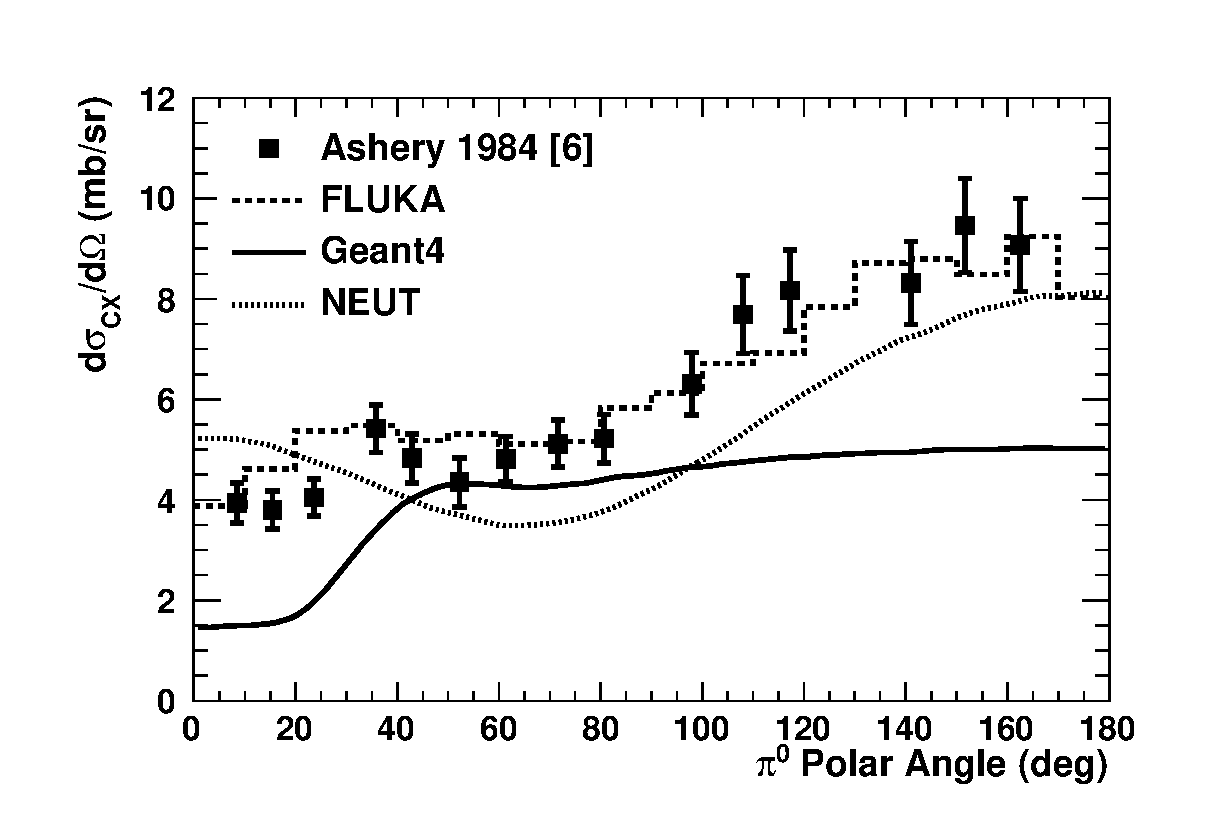
\includegraphics[width=86mm]{figures/dsigma_cx_o16_data_and_models.eps}
 \caption{$d\sigma_{\mathrm{CX}}/d\Omega$ as a function of the outgoing $\pi^0$ polar angle (in the lab frame) for 265 MeV$/c$ $\pi^{+}$ interacting on $^{16}$O, for \textsc{Fluka} (dashed line), \textsc{Geant4} (solid line) and \textsc{NEUT} (dotted line), along with data from \cite{Ashery2}.}
 \label{fig:pi0kinem}
\end{figure}

The modeling of the multiplicity and kinematics for nucleons ejected following an ABS or CX interaction show even larger discrepancies among models. The mechanisms for these processes are further complicated by the possibility of FSI of the nucleons before they exit the nucleus. Data on light nuclei that would help in the understanding and tuning of these processes are very scarce. \textsc{Neut} uses nucleon multiplicities published by \cite{Rowntree} of $\sigma_{\mathrm{ABS}}$ on N and Ar targets, but it is unclear what other models use.
%Despite the high purity of the events selected for this analysis, the effect of various models to our background prediction was investigated.
